\documentclass[12pt]{article}
\usepackage{amsmath}
\usepackage{amssymb}
\usepackage{geometry}
\usepackage{enumerate}
\usepackage{natbib}
\usepackage{float}%稳定图片位置
\usepackage{graphicx}%画图
\usepackage[english]{babel}
\usepackage{a4wide}
\usepackage{indentfirst}%缩进
\usepackage{enumerate}%加序号
\usepackage{multirow}%合并行
\title{Final Report}

\begin{document}
\maketitle
\newpage
\section{Search Algorithm}
\subsection{Room Segment}
The general function of the base board is moving to your appointed destination and return. To realize it, we cut the room into many small squares with coordinates. Then, we can tell  the coordinates of the destination. In addition, since the coordinate system is absolute, Metbin also should know the coordinates of its initial place to calculate its relative position about the destination.
\begin{figure}[H]
\centering
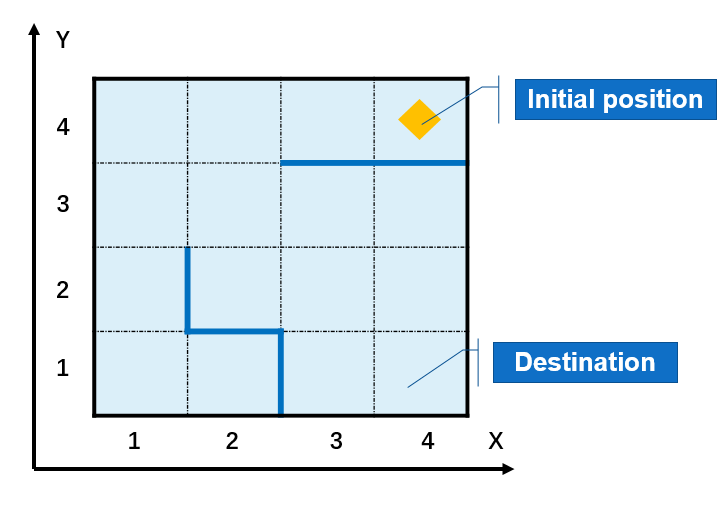
\includegraphics[scale=0.8]{P1.jpg}
\caption{Room segment with coordinates}
\end{figure}
In the figure 1, the room is cut into $4\times4$ squares with coordinates, and there are x and y axis. So we can know the initial position of Metbin is (4,4) and the destination's coordinates are (4,1). 
\subsection{Direction of Metbin}
Since we use a search algorithm, Metbin must know its direction relative to x and y axis, so it can know towards which square it's moving. Since the room is cut into squares, so we introduce a direction variable \textbf{d} of four values to represent robot's current direction. 
\begin{figure}[H]
\centering
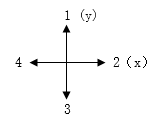
\includegraphics[scale=1]{P2.jpg}
\caption{Direction variable}
\end{figure}
The figure shows the direction in the room. Since its also absolute, it should be input to the Metbin in advance. We set the direction parallel to y axis is 1, and it will become plus one after Metbin turn right 90 degrees, and it will minus 1 after it turn left. It is worth to mention that \textbf{d} only has 4 values (1$\sim$4), so when its reaches 5, it will minus 4.
Similarly, when \textbf(d) is smaller than 1, it will plus 4.
\par In the figrue 1, it's clear that Metbin can only move against the direction of x axis, so its initial \textbf{d} is 4.
\subsection{Square Information and its Variables}
To realize the search function, we introduce ten variables to describe each square.
\begin{table}[H]
\centering
\begin{tabular}{|c|c|c|c|}
\hline
variable name & meaning  & value range  \\ \hline
\textbf{E} &The order of the square first reached by Metbin  & 1$\sim$16   \\ \hline
\textbf{X[E]} &The x coordinate of square \textbf{E}  &  1$\sim$4  \\ \hline
\textbf{Y[E]} &The y coordinate of square \textbf{E}  &  1$\sim$4  \\ \hline
\textbf{D[E]} &Metbin's \textbf{d} when it first reaches square \textbf{E}  &1$\sim$4    \\ \hline
\textbf{L[E]} &The left obstacle situation when Metbin first reaches square \textbf{E}  &-1$\sim$16  \\ \hline
\textbf{F[E]} &The front obstacle situation when Metbin first reaches square \textbf{E}  &-1$\sim$16     \\ \hline
\textbf{R[E]} &The right obstacle situation when Metbin first reaches square \textbf{E}  &-1$\sim$16     \\ \hline
\textbf{l[E]} &The left priority when Metbin reach square \textbf{E}  &0$\sim$3     \\ \hline
\textbf{f[E]} &The front priority when Metbin reach square \textbf{E}  &0$\sim$3     \\ \hline
\textbf{r[E]} &The right priority when Metbin reach square \textbf{E}  &0$\sim$3    \\ \hline
\end{tabular}
\caption{Variables describing a square}
\end{table}
\subsubsection{Square Order \textbf{E} and Direction \textbf{D[E]}}
As mentioned in table 1, \textbf{E} represents the order of the square first reached by Metbin. For example, in Figure 1, Metbin's initial position's \textbf{E} is 1 and the square with coordinates (3,4) is 2. Every square only has one corresponding \textbf{E}. If Metbin return a square which already has \textbf{E}, it won't change. Since there are 16 squares in the field, $E_{max}=16$.
\par Additionally, when Metbin first reaches the square, its \textbf{d} will be recorded as square \textbf{E}'s \textbf{D[E]}. It also won't change later.  
\subsubsection{Obstacle situation \textbf{L[E]}, \textbf{F[E]}, and \textbf{R[E]}}
As mentioned the before, the three variable describe the obstacle situation in three sides when Metbin is in the square with direction \textbf{D[E]}. If there is an obstacle on right side, then \textbf{R[E]} will be 0. If there is no obstacle then, if there is a reached square \textbf{E'}, then \textbf{R[E]}=\textbf{E'}, else ]\textbf{R[E]}=-1. Since there are 16 squares in the field, the obstacle variable can't be bigger than 16.  
\par If every square's obstacle situation is bigger than -1, than Metbin has already reached every squares.
\subsubsection{Priority Variable \textbf{l[E]}, \textbf{f[E]}, and \textbf{r[E]}}
The three variable in lower case describe the order of directions to turn when Metbin reach \textbf{E} with \textbf{D[E]}. These variable value is smaller than 3 because there is only 3 directions Metbin can advance. Metbin will choose the biggest variable and go its corresponding direction. 
\par For example , if Metbin reaches square \textbf{5} and \textbf{l[5]}=0, \textbf{f[E]}=1, and \textbf{r[5]}=3, then it will turn right keep going. Then \textbf{r[5]} will become 0 after Metbin go back.
\par When Metbin reaches a new square, the three variables will generated according to Metbin's relative location to the destination and obstacle situation variables. If there is an obstacle on the left side (\textbf{L[E]}=0) then \textbf{l[E]} will also be 0 because there can't go. If there is no wall, then if the obstacle is in front of Metbin, then \textbf{f[E]} will be 3. Then if the obstacle is on the right, \textbf{r[E]} will be 2 and \textbf{l[E]}=1. If the obstacle is on the back of Metbin, then \textbf{f[E]} will be 1 and other two variables will plus one correspondingly. Otherwise, Metbin will go at the order of left, front, then right.
\subsubsection{An Example without return from Figure 1}
\begin{figure}[H]
\centering
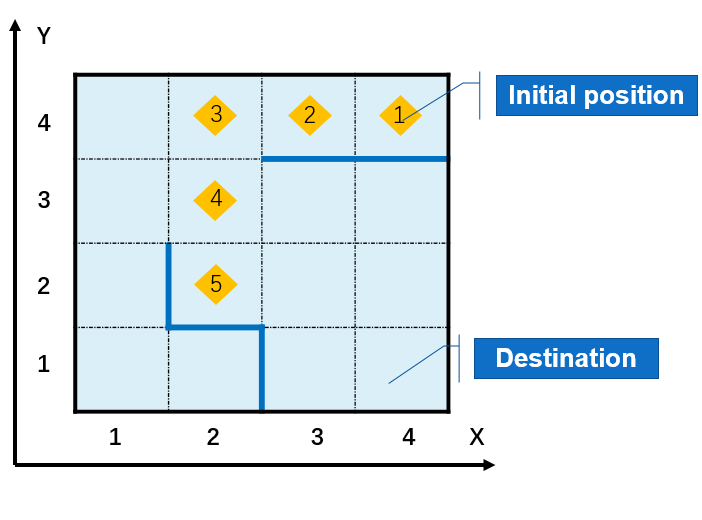
\includegraphics[scale=0.4]{P3.jpg}
\caption{Direction variable}
\end{figure}
The first 5 squares' \textbf{E} is already shown on the picture and the following table shows the information recorder when Metbin first reaches square 5.
\begin{table}[H]
\centering
\begin{tabular}{|c|c|c|c|c|c|c|c|c|c|}
\hline
\textbf{E}&\textbf{X[E]}&\textbf{Y[E]}&\textbf{D[E]}&\textbf{L[E]}&\textbf{F[E]}&\textbf{R[E]}&\textbf{l[E]}&\textbf{f[E]}&\textbf{r[E]}\\ \hline
1 &4  &4  &4  &0 &2 &0 &0 &2 &0  \\ \hline
2 &3  &4  &4  &0 &3 &0 &0 &1 &0  \\ \hline
3 &2  &4  &4  &4 &-1&0 &3 &2 &0  \\ \hline
4 &2  &3  &3  &-1&5&-1 &2 &3 &1 \\ \hline
5 &2  &2  &3  &-1&0&0  &2 &0 &0 \\ \hline
\end{tabular}
\caption{Information variables of the first 5 squares.}
\end{table}
\begin{figure}[H]
\centering
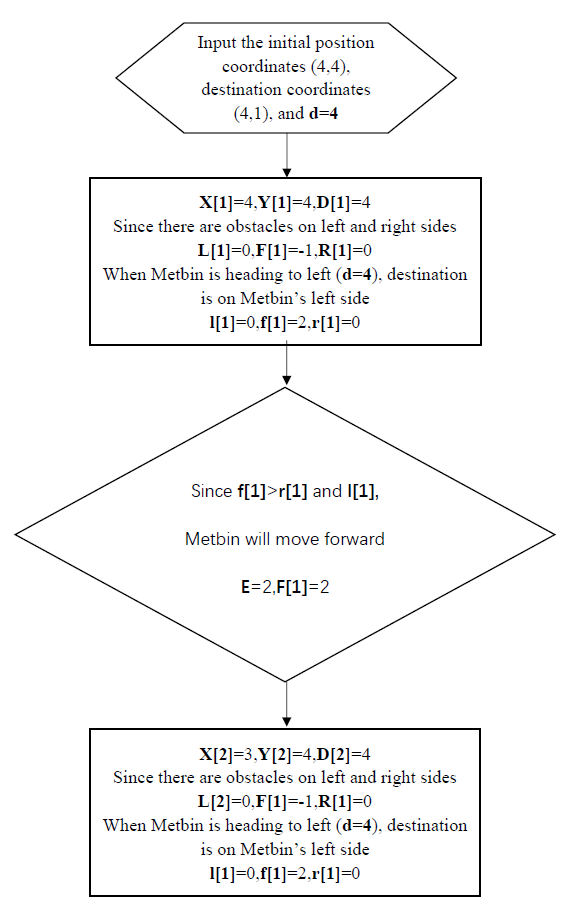
\includegraphics[scale=0.5]{P4.jpg}
\caption{Flow chart between square 1 and square 2}
\end{figure}
If there are only few obstacles, Metbin can go to the destination according to the above flow chart.
\begin{figure}[H]
\centering
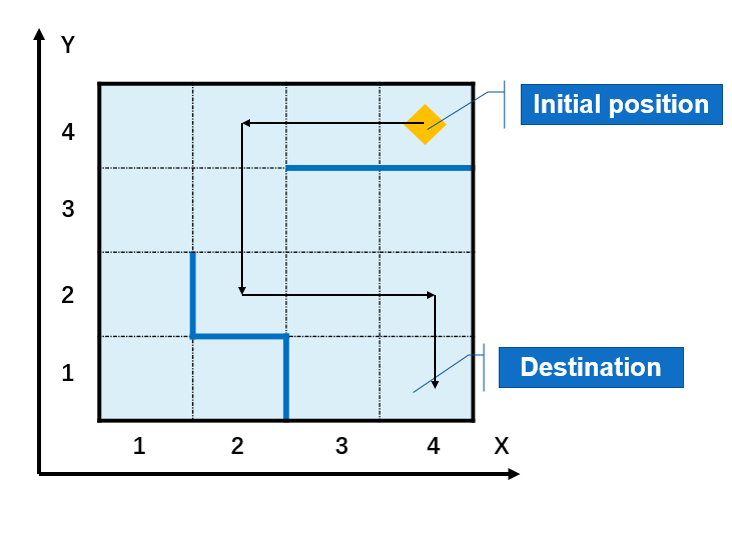
\includegraphics[scale=0.5]{P5.jpg}
\caption{Metbin's route to destination}
\end{figure}
\subsection{Realization of Return Function}
However, if there are many obstacles in the room, Metbin may reach a square \textbf{E} which has three walls around it (\textbf{L[E]}=0,\textbf{F[E]}=0, and \textbf{R[E]}=0). Then Metbin must return to another square \textbf{E'} who must have one obstacle situation variable equals to \textbf{E}. If there are many \textbf{E'} has such variable, then Metbin will go to the square with smallest \textbf{E'}.
\begin{figure}[H]
\centering
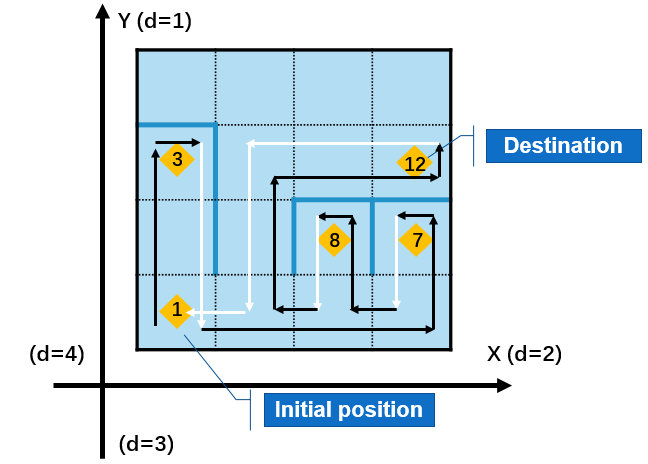
\includegraphics[scale=0.7]{P6.jpg}
\caption{Metbin's whole route in example 2}
\end{figure}
In the Figure 6, Metbin's initial square's coordinates are \textbf{X[1]}=1, \textbf{Y[1]}=1, and \textbf{D[1]}=1. The destination's coordinates are \textbf{X[E]}=4 and \textbf{Y[E]}=3. 
We draw the route of Metbin according to our algorithm, the black lines represent Metbin's route to a new square and the white lines represent its route of returning. Some square's \textbf{E} are already shown on the figure. This will be recorded when Metbin's moving. In this field, square \textbf{3}, \textbf{7}, and \textbf{8} has three obstacles around it, so Metbin will return after reached these squares. In addition, since the destination's coordinates has already been input to Metbin and it keeps recording its own coordinates. When these coordinates are same, Metbin knows that it has reached the destination and return.
\section{Computer Simulation}
Since the algorithm is hard to realize, we decide to simulate it on computer first. In this procedure, we draw a field and Metbin's route. Then we input the obstacle situation variable according to Metbin's route. This will be detected by infra-red sensors in real field. We only input 0 or -1 as every square's obstacle situation variable's value. (-1 means there is no obstacle and 0 represents there is an obstacle.)
\par for example in figure 6, we can input the following list
\begin{table}[H]
\centering
\begin{tabular}{|c|c|c|c|}
\hline
\textbf{E}  & \textbf{L[E]} & \textbf{F[E]} & \textbf{R[E]} \\ \hline
1  & 0        & -1       & -1       \\ \hline
2  & 0        & -1       & 0        \\ \hline
3  & 0        & 0        & 0        \\ \hline
4  & -1       & -1       & 0        \\ \hline
5  & -1       & -1       & 0        \\ \hline
6  & -1       & 0        & 0        \\ \hline
7  & 0        & 0        & 0        \\ \hline
8  & 0        & 0        & 0        \\ \hline
9  & 0        & -1       & 0        \\ \hline
10 & 0        & -1       & -1       \\ \hline
11 & -1       & -1       & 0        \\ \hline
12 & -1       & 0        & 0        \\ \hline
\end{tabular}
\caption{Input of Obstacle Situation}
\end{table}
Then the Metbin can generate every square's information variable according table 3
\begin{table}[H]
\centering
\begin{tabular}{|c|c|c|c|c|c|c|c|c|c|}
\hline
\textbf{E}  & \textbf{X[E]}  & \textbf{Y[E]} & \textbf{D[E]} & \textbf{L[E]} & \textbf{F[E]} & \textbf{R[E]} & \textbf{l[E]} & \textbf{f[E]} & \textbf{r[E]} \\ \hline
1  & 1        & 1        & 1        & 0        & 2        & 4        & 0        & 3        & 2        \\ \hline
2  & 1        & 2        & 1        & 0        & 3        & 0        & 0        & 3        & 0        \\ \hline
3  & 1        & 3        & 1        & 0        & 0        & 0        & 0        & 0        & 0        \\ \hline
4  & 2        & 1        & 2        & 9        & 5        & 0        & 2        & 3        & 0        \\ \hline
5  & 3        & 1        & 2        & 8        & 6        & 0        & 2        & 3        & 0        \\ \hline
6  & 4        & 1        & 2        & 7        & 0        & 0        & 3        & 0        & 0        \\ \hline
7  & 4        & 2        & 1        & 0        & 0        & 0        & 0        & 0        & 0        \\ \hline
8  & 3        & 2        & 1        & 0        & 0        & 0        & 0        & 0        & 0        \\ \hline
9  & 2        & 2        & 1        & 0        & 10       & 0        & 0        & 3        & 0        \\ \hline
10 & 2        & 3        & 1        & 0        & -1       & 11       & 0        & 2        & 3        \\ \hline
11 & 3        & 3        & 2        & -1       & 12       & 0        & 2        & 3        & 0        \\ \hline
12 & 4        & 3        & 2        & -1       & 0        & 0        & 0        & 0        & 0        \\ \hline
\end{tabular}
\caption{Information variable}
\end{table}
To test whether Metbin will move according to the correct route, we introduce a array \textbf{A[i]} of four values from $1\sim3$. 
\begin{table}[H]
\centering
\begin{tabular}{|c|c|c|c|}
\hline
\textbf{A[i]} & 1                           & 2                    & 3                     \\ \hline
         & move forward to next square & turn left 90 degrees & turn right 90 degrees \\ \hline
\end{tabular}
\caption{Array \textbf{A}}
\end{table}
So Metbin should generate \textbf{A[i]=$\lbrace 11133111333111212213133212213133211311221121131\rbrace$}
if the Metbin can generate the correct \textbf{A[i]} according to our input obstacle information, we just need to let Metbin read the array and make the correct motion
\section{Realization of \textbf{A[i]}} 
Since the environment is of great randomness, we must use multiple sensors to ensure Metbin is in the correct position in the field. We decide to use posture sensors, encoders and many infra-red sensors.
\subsection{Posture Sensors}
The posture sensors have many functions such as detect the magnetic field and its angle. It can calculate its deflection angle by angular acceleration integral and this is the only function required. so I can set it on computer.
\begin{figure}[H]
\centering
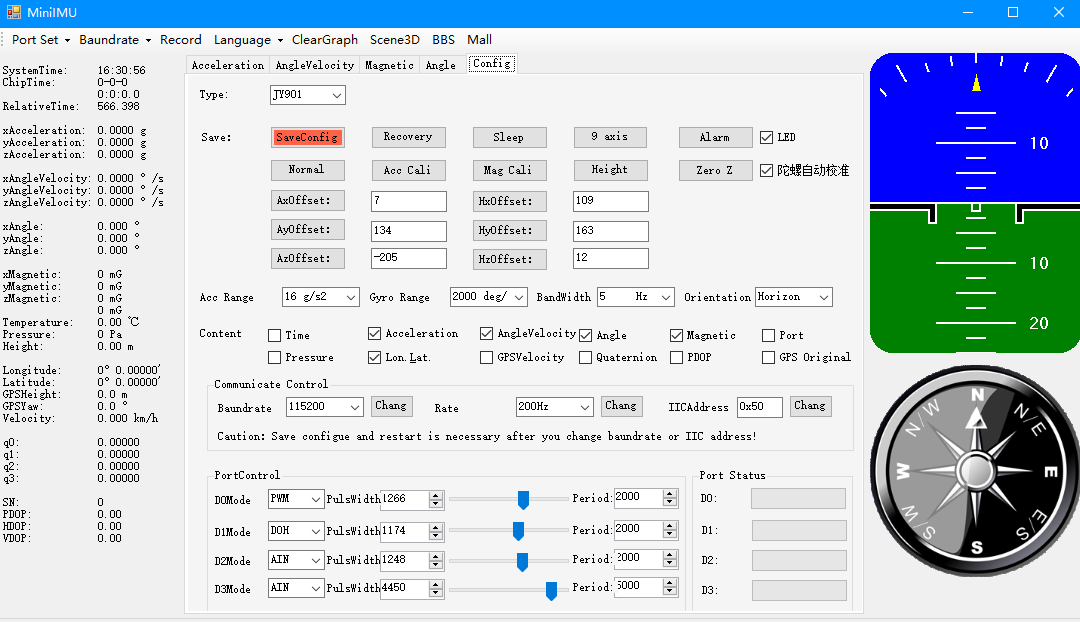
\includegraphics[scale=0.5]{P7.jpg}
\caption{Posture Sensors' setting surface on computer}
\end{figure}
The posture sensors can return a value \textbf{z} describing the angle deflected. It's value range is $0\sim360$. If the Metbin needs to turning right 90 degrees, it will only turn until \textbf{z}-\textbf{$\mathbf{z_{initial}}$}$\approx90^o$. Similarly to \textbf{d} in Search Algorithm, $\mathbf{\bigtriangleup_z}$ may be small than 0 sometime, so it need to be dealt with. 
\subsection{Encoders}
We use encoders to recorded how far does Metbin move on the field. To eliminate accumulative, it will be set to 0 every time Metbin meet an obstacle. The encoders can return 1 and 0 when it receive a change in Motor's voltage. So we can record the number of pulse to calculate how far does Metbin move. After many experiments, we think when Metbin will move 55cm when 1500 pulse are returned.
\subsection{Infra-red Sensors}
Infra-red sensors can return its distance from obstacle. 
\begin{figure}[H]
\centering
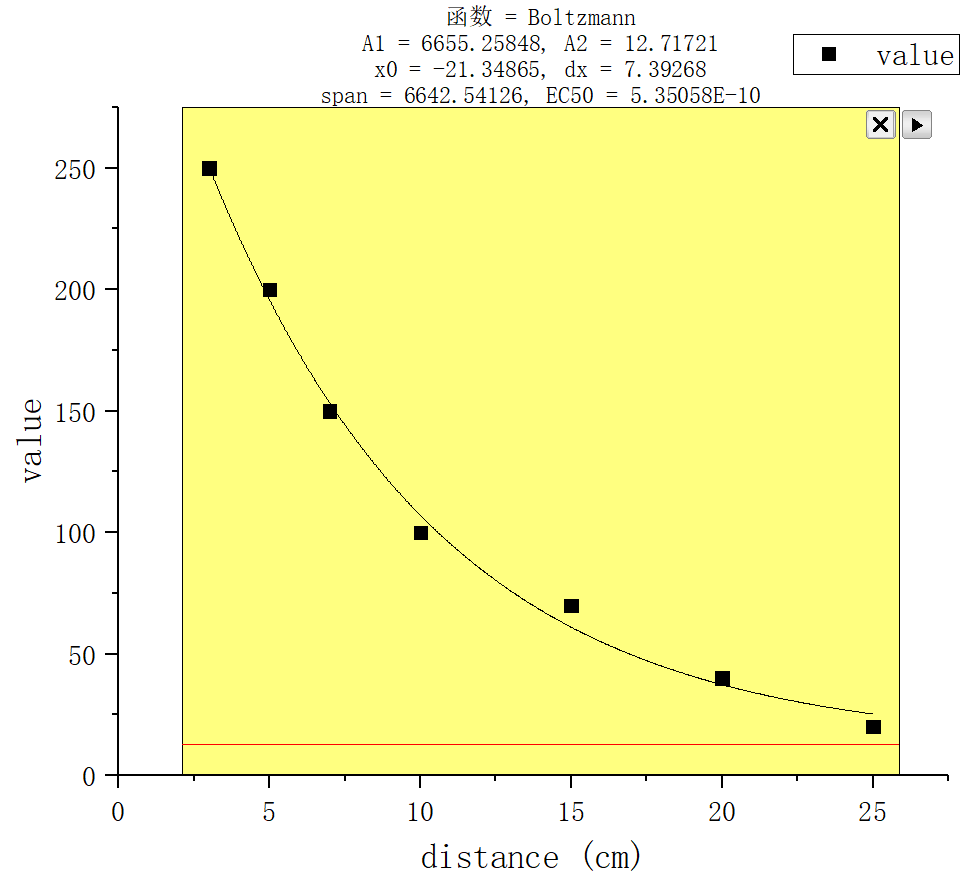
\includegraphics[scale=0.5]{P8.jpg}
\caption{Relation between the distance and return value. }
\end{figure}
When infra-red sensors' return value is bigger than 100, we assume there is an obstacle before it. We install five infra-red sensors on Metbin, one is installed at the head and two are installed at left and right sides respectively. In addition ,infra-red sensors can be used to detect whether Metbin is parallel to the wall. Since there are two infra-red sensors on one side. If $\frac{v_1-v_2}{v_1+v_2}<0.01$ then Metbin is parallel to the wall. The posture's accumulative error will be eliminate at the time.
\end{document}